% Compile twice with pdfLaTeX from this directory.
% English slides, with speaker notes and timing in each frame.
% Define \presenternotes before input to produce a notes-only PDF.
\documentclass[aspectratio=1610,xcolor=dvipsnames,t]{beamer}
\usepackage{lmodern}
\usepackage{sansmath}
\usepackage{mathastext}
\usepackage{graphicx}
\usepackage{beamerthemesplit}
\usetheme[compress]{Heidelberg}
\definecolor{unirot}{rgb}{0.5976525,0,0}
\usecolortheme[named=unirot]{structure}
\usepackage{amsmath,amssymb}
\newcommand{\toprule}{\hline}
\newcommand{\midrule}{\hline}
\newcommand{\bottomrule}{\hline}
\setbeamertemplate{headline}{}
\ifdefined\presenternotes
  \setbeameroption{show only notes}
\else
  \setbeameroption{hide notes}
\fi
\newcommand{\keyterm}[1]{\textcolor{unirot}{\textbf{#1}}}
% Keep existing backup content while suppressing per-slide source labels.
\newcommand{\papersource}[1]{}
\newcommand{\paperfig}[4][.50\textheight]{%
  \includegraphics[page=#2,viewport=#3,clip,width=#4,height=#1,keepaspectratio]{../2408.03314v1.pdf}}
\title[Test-Time Compute in LLMs]{Scaling LLM Test-Time Compute Optimally can be More Effective than Scaling Model Parameters}
\subtitle{Allocating inference compute under a fixed budget}
\author[Zhenbang Lyu]{Zhenbang Lyu}
\institute[Uni HD]{Heidelberg University\\Institute of Computer Science}
\date[]{Charlie Snell, Jaehoon Lee, Kelvin Xu, and Aviral Kumar\\2024, arXiv:2408.03314v1}

\begin{document}

\begin{frame}[plain]
  \titlepage
  \note{Time 0:00--0:30. The paper asks how to improve a fixed model by spending more computation when it answers a question. We will first examine how to allocate that computation, then compare it with training a larger model.}
\end{frame}

\begin{frame}{Can Thinking Longer Improve an Answer?}
  A bat and a ball cost \$1.10 in total. The bat costs \$1.00 more than the ball. How much does the ball cost?
  \par\medskip
  \begin{itemize}
    \item \textbf{A quick guess}\quad The ball costs \$0.10. But then the bat costs \$1.10, giving a total of \$1.20.
    \item \textbf{After checking}\quad Let the ball cost $x$. Then $x+(x+1)=1.10$, so the ball costs \$0.05.
  \end{itemize}
  \par\medskip
  Extra thought helps us check and revise an initial answer.
  \par\smallskip
  \keyterm{Can a trained language model benefit in a similar way?}
  \note{Time 0:30--1:30. Use this illustrative arithmetic puzzle to make the paper's human-thinking motivation concrete. An intuitive answer can fail a simple check. Spending more effort on the same question can recover a correct answer without acquiring new knowledge. This illustrates a possibility, rather than a guarantee that thinking longer always helps. The example is an introduction for this talk. Next explain what extra effort means operationally for a model.}
\end{frame}

\begin{frame}{How Can a Model Use More Computation?}
  For a model, extra effort means more computation while answering, after training: \textbf{test-time compute}.
  \par\smallskip
  Suppose the budget allows 16 candidate answers to a math problem.
  \par\medskip
  \begin{itemize}
    \item Generate 16 independent attempts and select an answer.
    \item Generate a chain of 16 attempts, each conditioned on earlier answers.
    \item Spend the budget searching over partial solutions with a verifier.
  \end{itemize}
  \par\medskip
  \keyterm{Which allocation gives the highest chance of a correct final answer?}
  \par\medskip
  Each option needs a way to generate candidates and a way to choose among them.
  \note{Time 1:30--2:15. Connect checking and revising the human answer with concrete operations for a model. Keep the same model and question while comparing independent attempts, revisions, and verifier-guided search. Sixteen candidates are an illustrative budget. All three need generation and evaluation, which motivates the proposer/verifier framework on the next slide.}
\end{frame}

\begin{frame}{The Proposer and Verifier Framework}
  The paper describes these choices through two components.
  \par\smallskip
  \begin{description}
    \item[Proposer] The language model generates candidate solutions from a probability distribution.
    \item[Verifier] A learned model scores candidates or partial solutions.
  \end{description}
  \par\medskip
  \begin{itemize}
    \item \keyterm{Revisions} change the proposal distribution by including earlier answers in the next input.
    \item \keyterm{Verifier-guided search} uses scores to select candidates or decide which prefixes to expand.
  \end{itemize}
  \par\medskip
  We will examine both routes, then ask whether a small model using them can outperform a larger model at equal total FLOPs.
  \note{Time 2:15--3:15. Connect proposer to generating attempts and verifier to judging them. Distribution means the probabilities of different responses. Feeding back an earlier answer changes these probabilities. Revisions can also use a verifier for final selection. Establish the order of the talk: search, revisions, then a comparison with larger models.}
\end{frame}

\begin{frame}{Experimental Setup}
  To test these ways of using extra computation, the authors study mathematical reasoning.
  \par\smallskip
  \begin{itemize}
    \item \textbf{Task}\quad MATH, high-school competition mathematics with a range of difficulty levels.
    \item \textbf{Data split}\quad 12,000 training questions and 500 test questions.
    \item \textbf{Base model}\quad PaLM 2-S* (Codey), with task-specific fine-tuning for verification and revision.
  \end{itemize}
  \par\medskip
  The model already solves some problems. We now need to decide how much exploration or refinement each question needs.
  \note{Time 3:15--4:00. The model and task give a concrete test of the opening question. The model already has relevant knowledge but has not saturated on MATH. Verification and revision capabilities require task-specific training. We next need a rule for allocating computation across questions.}
\end{frame}

\begin{frame}{Choosing a Strategy by Difficulty and Budget}
  A promising first answer may benefit from revision. A poor starting point may need a fresh attempt.
  \par\smallskip
  The authors use \keyterm{difficulty relative to the base model} to choose settings for each budget.
  \par\medskip
  \begin{enumerate}
    \item Estimate difficulty from 2,048 independent samples per question.
    \item Sort questions into five equal-frequency bins, from easy to hard.
    \item For each bin and budget, select a setting on one fold and evaluate on the other. Swap folds and average.
  \end{enumerate}
  \par\smallskip
  \begin{tabular}{@{}ll@{}}
    \textbf{Oracle bins} & Rank by actual correctness rate.\\
    \textbf{Predicted bins} & Rank by the verifier's mean final-answer score.
  \end{tabular}
  \par\medskip
  \keyterm{Reported budgets exclude difficulty-estimation cost.}
  \note{Time 4:00--5:30. The formal goal is to maximize the probability of a correct final answer for a question and budget. Exact per-question success rates are unknown, so difficulty is a proxy. Oracle and predicted scores produce separate partitions. Two-fold validation separates choosing a strategy from evaluating it. Difficulty-estimation cost is excluded. We now apply this allocation rule to the first route: search guided by a verifier.}
\end{frame}

\begin{frame}{Training a Process Reward Model}
  To choose which partial solutions to develop, search needs a score for each prefix.
  \par\smallskip
  A \keyterm{process reward model (PRM)} estimates the chance of eventual success under the base model's sampling policy.
  \par\medskip
  \begin{itemize}
    \item Keep a solution prefix through the current step.
    \item Sample multiple continuations to completion and check final correctness.
    \item Use the success rate as a training target for the PRM.
  \end{itemize}
  \par\medskip
  Illustrative training target: 7 correct completions out of 10 gives $0.7$.
  \par\smallskip
  \begin{itemize}
    \item Their PRM outperformed an outcome reward model (ORM) baseline, so subsequent search experiments use the PRM.
  \end{itemize}
  \note{Time 5:30--7:00. Monte Carlo rollouts create supervision before the search experiments. A label of 0.7 estimates future success from the whole prefix under this base model. The trained PRM can then predict such values directly. ORM scores complete outcomes. The paper reports that their PRM performs better. Mention that the authors suspect distribution shift between GPT-4 solutions in PRM800k and PaLM 2 outputs.}
\end{frame}

\begin{frame}{PRM Scores and Final Answer Selection}
  Training gives us scores for partial solutions. We also need a rule for choosing the final answer when candidates are complete.
  \par\smallskip
  \textbf{Within a solution}\quad Use the PRM score at its last step as the full-solution score.
  \par\medskip
  \textbf{Across solutions}\quad Weighted best-of-$N$ sums scores for candidates with the same final answer.
  \par\medskip
  \centering
  \begin{tabular}{lcc}
    \toprule
    Example candidate & Final answer & Full-solution score\\
    \midrule
    1 & $x=2$ & 0.60\\
    2 & $x=2$ & 0.55\\
    3 & $x=3$ & 0.90\\
    \bottomrule
  \end{tabular}
  \par\par\medskip
  $x=2$: $0.60+0.55=1.15$\qquad $x=3$: $0.90$
  \par\par\smallskip
  Weighted selection returns $x=2$. Majority voting counts occurrences without these weights.
  \note{Time 7:00--8:15. Distinguish training a scorer from deciding how to use its scores. The last-step score uses the entire solution prefix. The aggregate 1.15 is a sum of scores, not a probability. Standard best-of-N would choose the single highest-scoring candidate here. Weighted best-of-N pools support for the same final answer. Majority also groups identical answers, but gives every candidate equal weight.}
\end{frame}

\begin{frame}{Search Methods with a PRM}
  The same scorer can evaluate complete answers or guide generation before a solution is finished.
  \begin{center}
    \paperfig[.54\textheight]{8}{61 493 551 710}{.98\textwidth}
  \end{center}
  \small
  \textbf{Best-of-$N$}\quad Complete independent candidates, then score.\\
  \textbf{Beam search}\quad Score prefixes, retain top candidates, expand again.\\
  \textbf{Lookahead}\quad Continue $k$ steps temporarily before scoring a prefix. Its extra rollout also consumes budget.
  \note{Time 8:15--10:00. Link final selection to the simplest method, independent complete candidates. Beam search brings scoring into the generation process. With N=6 and M=2, score six prefixes, retain three, and extend each twice. Lookahead evaluates a prefix by temporary greedy continuation of up to k steps. k=0 gives beam search and its cost is approximately N(k+1). Having defined the alternatives, compare their accuracy at matched budgets.}
\end{frame}

\begin{frame}{Search Results Depend on Budget and Difficulty}
  \begin{center}
    \paperfig[.52\textheight]{9}{61 539 551 708}{.98\textwidth}
  \end{center}
  \small
  \begin{itemize}
    \item Low budgets favor beam search. At higher budgets, its advantage shrinks.
    \item Breaking down by difficulty explains the difference: easy bins 1--2 can deteriorate as search exploits PRM errors, while beam search helps in bins 3--4.
    \item The hardest bin improves little. Lookahead usually trails at matched cost.
  \end{itemize}
  \note{Time 10:00--12:00. Read the left graph first: x is generation budget, y is MATH accuracy. Stronger search can exploit an imperfect scorer. The right graph groups questions by difficulty and bars reflect increasing budgets. Medium bins benefit, while easy bins can degrade. Search sometimes produces repetitive steps and overly short answers. These different outcomes explain why the difficulty-based rule introduced earlier is useful.}
\end{frame}

\begin{frame}{Difficulty-Based Allocation Improves PRM Search}
  \begin{columns}[T,onlytextwidth]
    \begin{column}{.59\textwidth}
      \centering
      \paperfig[.65\textheight]{10}{306 466 551 635}{\linewidth}
    \end{column}
    \begin{column}{.38\textwidth}
      \small
      Since different settings win in different bins, select the best search setting for each bin and budget.
      \par\medskip
      At low budgets, 16 generations nearly match best-of-$N$ with 64.
      \par\medskip
      With predicted bins, some gains diminish at higher budgets.
      \par\medskip
      Can we also improve what the model proposes by letting it revise earlier answers?
    \end{column}
  \end{columns}
  \note{Time 12:00--13:00. Apply the earlier policy to search. Separate oracle from predicted difficulty. Low-budget adaptive search approaches best-of-N using one-quarter of the generation budget. At high budgets, predicted-difficulty gains diminish. We have improved which candidates receive computation. Next we change how the model generates its next candidate, by teaching it to revise earlier answers.}
\end{frame}

\begin{frame}{Training and Running a Revision Model}
  The second route lets the generator use earlier answers to produce a better next attempt.
  \par\smallskip
  \textbf{Training data}
  \begin{itemize}
    \item Generate 64 independent answers per training question at higher temperature.
    \item Pair a correct target with 0--4 incorrect answers, prioritizing related text using character edit distance.
    \item Fine-tune the model to produce the correct target given the question and earlier answers.
  \end{itemize}
  \par\medskip
  \textbf{At inference}
  \begin{itemize}
    \item Generate a chain, keeping the most recent four answers in context.
    \item Revisions can undo correct answers. Select among candidates using a verifier or majority vote.
  \end{itemize}
  \note{Time 13:00--14:15. Contrast selecting promising prefixes with generating a new full solution conditioned on earlier answers. The 64 independent training answers form synthetic trajectories afterward. Edit distance favors related incorrect context and correct targets. At inference, retain only the most recent four in input while storing all candidates. Training context contained incorrect answers, so the model may undo a correct answer. The reported rate is about 38 percent under naive revision. Final selection addresses this risk. Next test whether the revision model actually improves outputs.}
\end{frame}

\begin{frame}{Revision Quality and Final Answer Accuracy}
  \begin{center}
    \paperfig[.48\textheight]{12}{61 539 551 715}{.98\textwidth}
  \end{center}
  \small
  \begin{itemize}
    \item \textbf{Left}\quad Single-answer accuracy improves overall with revision, then fluctuates around a plateau.
    \item \textbf{Right}\quad At the same candidate count, sequential generation generally beats parallel generation with either selection method.
  \end{itemize}
  \par\smallskip
  Could several independent revision chains work better than one long chain?
  \note{Time 14:15--16:00. Left: average correctness at each fixed position across four 64-answer trajectories per question, then across questions. A 64-answer chain uses a four-answer context window. Right: after generating N candidates, measure the selected answer's correctness. Four curves cross generation with selection choices. Sequential generation generally wins. Independent starts still explore different approaches, so the next question is whether mixing parallel starts and sequential revisions works even better.}
\end{frame}

\begin{frame}{Combining Fresh Starts with Revisions}
  \begin{center}
    \paperfig[.51\textheight]{13}{61 539 551 708}{.98\textwidth}
  \end{center}
  \small
  \begin{itemize}
    \item With 16 candidates: 16 chains of length 1, four of length 4, or one of length 16.
    \item \textbf{Left}\quad Each line fixes the budget. Moving right puts more compute into each chain.
    \item \textbf{Right}\quad At 128 candidates, easy bins favor long chains. Harder bins can favor a mixture.
  \end{itemize}
  \note{Time 16:00--17:45. Chain length times independent chain count is the candidate budget. Their ratio is the horizontal axis. In the combined strategy, the verifier selects within chains and then across chains. Left colors encode budgets, right colors encode ratios. Easy questions favor long chains. Harder questions can benefit from multiple approaches. This gives us the same opportunity as search: choose the best configuration separately for each difficulty bin and budget.}
\end{frame}

\begin{frame}{Compute-Optimal Revisions Improve Scaling}
  \begin{columns}[T,onlytextwidth]
    \begin{column}{.59\textwidth}
      \centering
      \paperfig[.65\textheight]{13}{306 186 551 357}{\linewidth}
    \end{column}
    \begin{column}{.38\textwidth}
      \small
      Apply the same difficulty-based rule to the sequential/parallel ratio.
      \par\medskip
      Parallel sampling begins to plateau at high budgets.
      \par\medskip
      Adaptive revisions can beat parallel best-of-$N$ with 64 rather than 256 candidates.
      \par\medskip
      How far can these gains close the gap to a larger model?
    \end{column}
  \end{columns}
  \note{Time 17:45--18:45. Solid curves use weighted best-of-N, dashed curves use majority. Colors distinguish oracle policy, predicted policy, and pure parallel generation. The revisions-specific example compares 64 with 256 generations. Both method routes now show better use of a fixed model's inference compute. We can therefore return to the bigger question: could that gain replace some investment in training a larger model?}
\end{frame}

\begin{frame}{Pretraining and Inference at Equal Total FLOPs}
  Extra inference improves the small model. How does it compare with training a larger model?
  \par\smallskip
  Hold training tokens fixed and increase parameters by a factor $M$.
  \[
    X\approx6PD_{\mathrm{pretrain}},\qquad
    Y\approx2PD_{\mathrm{inference}}
  \]
  $P$ is the parameter count. $D_{\mathrm{inference}}$ is the total inference token workload.
  \par\medskip
  \[
    \underbrace{X+aY}_{\text{small model, extra inference}}
    =\underbrace{M(X+Y)}_{\text{large model, greedy decoding}}
  \]
  \par\medskip
  The larger model costs more both to train and to run. The small model can spend its training savings on inference.
  \note{Time 18:45--20:15. Move from choosing inference strategies to choosing where to spend the total compute budget. P denotes parameter count, distinct from earlier candidate count N. X and Y are the small model's baseline training and inference costs. The larger model costs M times as much for both, with training tokens fixed. The small model can use the training savings for more inference. We next calculate how much extra inference that buys.}
\end{frame}

\begin{frame}{Inference Workload Determines the Exchange Rate}
  \[
    R=\frac{D_{\mathrm{inference}}}{D_{\mathrm{pretrain}}},
    \qquad a=M+\frac{3(M-1)}{R}
  \]
  \begin{itemize}
    \item Low $R$: training savings are spread over fewer inference tokens, allowing more extra compute per request.
    \item High $R$: the same savings are spread across a larger inference workload.
  \end{itemize}
  \par\medskip
  \centering
  \begin{tabular}{lrrr}
    \toprule
    Workload & Low & Comparable & High\\
    \midrule
    $R$ & 0.16 & 0.79 & 22\\
    $a$, for $M\approx14$ & $\approx258$ & $\approx63$ & $\approx16$\\
    \bottomrule
  \end{tabular}
  \note{Time 20:15--21:30. Solve X+aY=M(X+Y) and use X/Y=3/R. a multiplies baseline inference compute. R counts the expected total inference workload. Low R concentrates training savings on fewer inference tokens. The same large model therefore has three different matched-budget comparison points. These are the three vertical lines in the next figure.}
\end{frame}

\begin{frame}{Small Model with Extra Compute versus Larger Model}
  \begin{center}
    \paperfig[.57\textheight]{15}{64 526 549 715}{.98\textwidth}
  \end{center}
  \small
  \textbf{Curves}\quad Small model with adaptive revisions (left) or PRM search (right).\\
  \textbf{Stars}\quad Greedy accuracy of the $\sim14\times$ larger model.\\
  Compare the same color at each workload's vertical line. A curve above its star favors additional inference. Colors use oracle difficulty bins.
  \note{Time 21:30--23:45. Difficulty colors match curves and stars. Stars repeat at three x positions, with the same y value, because matched compute differs by workload. For the left green curve, at low matched budget the star is higher, while at high matched budget the curve is higher. Easy/intermediate problems and low inference workload often favor extra inference. Hard problems and high workload often favor more pretraining. The result uses oracle difficulty and fixed training token counts.}
\end{frame}

\begin{frame}{Limits of the Comparison}
  \begin{itemize}
    \item Estimating difficulty needs substantial compute, excluded from reported budgets.
    \item Hardest problems gain little from the tested search and revision methods.
    \item The evidence comes from PaLM 2-S* on MATH, with capability-specific fine-tuning.
    \item The FLOPs comparison scales parameters at fixed training data and uses oracle difficulty bins.
  \end{itemize}
  \note{Time 23:45--24:30. Real deployment must pay for difficulty estimation. The data and model constrain generality. The larger-model comparison is one parameter-scaling setting. The paper leaves the combination of PRM tree search with revision chains for future study.}
\end{frame}

\begin{frame}{Conclusions}
  \begin{itemize}
    \item The best use of inference compute depends on both the question and the budget.
    \item Difficulty-based allocation improves PRM search and sequential/parallel revisions, with up to fourfold generation-budget savings in reported comparisons.
    \item Extra inference can substitute for larger models on some problems and workloads. The hardest problems remain a limitation.
  \end{itemize}
  \par\medskip
  \keyterm{The title's claim is conditional on problem difficulty and expected inference workload.}
  \note{Time 24:30--25:00. Return to the opening question. A fixed generation budget can be spent in very different ways. Choosing adaptively improves efficiency. The larger-model claim follows only under certain problem and workload conditions. End here at 25 minutes, excluding questions.}
\end{frame}

\begin{frame}{Questions}
  \vfill
  \begin{center}
    {\Huge\color{unirot}\textbf{Thank you}}\\[.4cm]
    {\Large Questions and Discussion}
  \end{center}
  \vfill
  \note{Questions begin after the 25-minute talk. Backup slides contain details on validation, rollouts, and FLOPs accounting.}
\end{frame}

\appendix

\begin{frame}{Backup: Difficulty Bins and Cross-Validation}
  \begin{enumerate}
    \item Score every question using 2,048 samples. Sort and divide into five quantiles.
    \item Within a bin, split questions into folds A and B.
    \item Use fold A to select settings at each budget. Evaluate those settings on B.
    \item Swap A and B. Average held-out performance.
  \end{enumerate}
  \par\medskip
  Oracle and predicted difficulty repeat this procedure with different scoring rules.
  \papersource{Section 3.2.}
  \note{Optional backup. Oracle uses actual correctness, predicted difficulty uses mean verifier scores. The bin boundaries are quantiles of scores across questions. A score such as 0.7 has no universal fixed bin.}
\end{frame}

\begin{frame}{Backup: Training Rollouts and Lookahead}
  \begin{description}
    \item[PRM training] Sample multiple continuations from a prefix to estimate expected final correctness. This supplies supervision.
    \item[Lookahead search] At inference time, generate up to $k$ extra steps with temperature 0. Use the trained PRM's score at that endpoint to evaluate the current prefix.
  \end{description}
  \par\medskip
  The temporary lookahead steps help choose which current prefixes to retain. Beam search is the $k=0$ case.
  \papersource{Sections 5.1--5.2.}
  \note{Optional backup. These two uses of rollout occur at different stages. Training rollouts create target values, while lookahead consults a trained PRM during search and incurs extra inference cost.}
\end{frame}

\begin{frame}{Backup: Deriving the Inference Multiplier}
  \[
    X+aY=M(X+Y)
  \]
  \[
    a=M+(M-1)\frac{X}{Y}
  \]
  \[
    \frac{X}{Y}=\frac{6PD_{\mathrm{pretrain}}}{2PD_{\mathrm{inference}}}
    =\frac{3}{R}
  \]
  \[
    \boxed{a=M+\frac{3(M-1)}{R}}
  \]
  Approximate FLOPs per token: forward $2P$, backward $4P$, training total $6P$.
  \papersource{Section 7.}
  \note{Optional backup. Backward computation forms gradients for weights and for activations, with each major matrix computation comparable to a forward pass. Total P includes parameters in every layer, so layer count is already accounted for. These approximations omit some operations.}
\end{frame}

\end{document}
